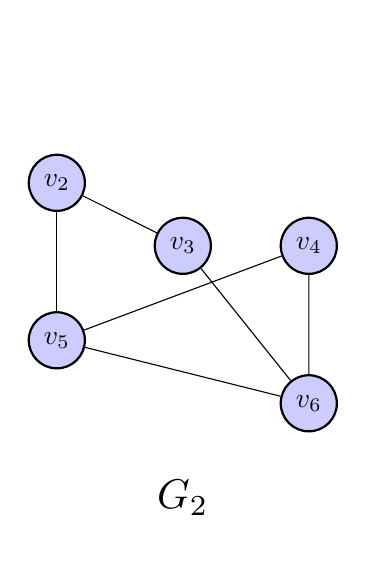
\begin{tikzpicture}
  [scale=.8,auto=left,every node/.style={circle,fill=blue!20,draw=black,thick}]
  \node (n1) at (3,6) [opacity=0] {$v_1$};
  \node (n2) at (1,4) {$v_2$};
  \node (n3) at (3,3) {$v_3$};
  \node (n4) at (5,3) {$v_4$};
  \node (n5) at (1,1.5) {$v_5$};
  \node (n6) at (5,0.5) {$v_6$};

  \foreach \from/\to in {n2/n3, n2/n5, n3/n6, n4/n5, n4/n6, n5/n6}
    \draw (\from) -- (\to);


   \node[draw=none, fill=none, scale=1.5] at (3,-1) {$G_2$};
\end{tikzpicture}
